%%% LaTeX Template
%%% This template is made for project reports
%%%	You may adjust it to your own needs/purposes
%%%
%%% Copyright: http://www.howtotex.com/
%%% Date: March 2011

%%% Preamble
\documentclass[paper=a4, fontsize=12pt]{scrartcl}	% Article class of KOMA-script with 12pt font and a4 format


\usepackage[english]{babel}				% English language/hyphenation
\usepackage[protrusion=true,expansion=true]{microtype}	% Better typography
\usepackage{amsmath,amsfonts,amsthm}			% Math packages
\usepackage[pdftex]{graphicx}				% Enable pdflatex
\usepackage{url}
\usepackage[margin=1.5in]{geometry}
\usepackage{algorithm}
\usepackage{algorithmic}
\usepackage{framed}
\usepackage{listings}

\lstset{
language=Matlab,
basicstyle=\footnotesize,
tabsize=2
}


%%% Custom sectioning (sectsty package)
\usepackage{sectsty}					% Custom sectioning (see below)
\allsectionsfont{\normalfont\scshape}			% Change font of al section commands


%%% Custom headers/footers (fancyhdr package)
\usepackage{fancyhdr}
\pagestyle{fancyplain}
\fancyhead{}						% No page header
%\fancyfoot[L]{\small \url{HowToTeX.com}}		% You may remove/edit this line 
\fancyfoot[C]{}						% Empty
\fancyfoot[R]{\thepage}					% Pagenumbering
\renewcommand{\headrulewidth}{0pt}			% Remove header underlines
\renewcommand{\footrulewidth}{0pt}			% Remove footer underlines
\setlength{\headheight}{13.6pt}


%%% Equation and float numbering
\numberwithin{equation}{section}		% Equationnumbering: section.eq#
\numberwithin{figure}{section}			% Figurenumbering: section.fig#
\numberwithin{table}{section}				% Tablenumbering: section.tab#


%%% Maketitle metadata (Defines how everything above the body should look like: title, header, authors, date, etc..)
\newcommand{\horrule}[1]{\rule{\linewidth}{#1}} 	% Horizontal rule

\title{
\vspace{-1in} 	
\usefont{OT1}{bch}{b}{n}
\normalfont \normalsize \textsc{University of Edinburgh - School of Informatics}
\\ [25pt]
\horrule{0.5pt} \\[0.4cm]
\large IAR - Task 2 Report \\
\horrule{1pt} \\[0.5cm]
}
\author{
  \normalfont \normalsize
  Jakob Calero - s0948339\\[-3pt]\normalsize
  Samuel Neugber - s0821562\\[-3pt]\normalsize
  \today
}
\date{}


%%% Begin document
\begin{document}
\maketitle					% Insert the title here
\section{Abstract}
A dynamically changing task usually requires a dynamic solution. In this task we are asked to follow a dynamically moving light source while avoiding obstacles in an arena. We have therefore revisited the approach of setting motor speeds as a direct function of the sensor values and assuming obstacle detection from the same conditional approach we used in our previous task. The robot will move towards a sufficiently close lightsource in a smooth trajectory while at the same time avoiding obstacles.

\section{Introduction}
In the last task we explored two different control methods for our robot: one which acted on certain threshold-conditions of the infra-red (IR) sensors, and one which directly mapped the values from the sensors to motor speeds. Our findings were that the first approach (conditional control) works well enough in relatively static environments and is a little easier to reason about than the other approach.

This task, on the other hand, required our robot to exhibit more dynamic behaviour in order to follow a light which could frequently change its position. We therefore went back and changed the control method to a more direct function between sensor values and motor control as in our second method in the last task. Using the photo sensors on the robot we calculate a relative angle it should be facing and that angle is then taken as input to the functions which detemine the speed of the individual wheels. The obstacle detection is handled by a conditional approach based on the IR sensors and is taken as higher priority than approaching the light source.

\section{Methods} 
\subsection{Light Direction Detection}
\label{LDD}
Our robot has 8 sensors detecting levels of light at a value range of 0 to 500, which are arranged as seen in (\emph{figure \ref{fig:img_sensors}}). From this information we ultimately want to estimate a direction the light could be originating from by combining the values and orientations of the individual sensors.

\begin{figure}[h!]
 \centering
  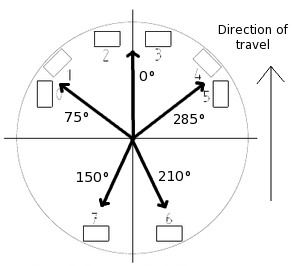
\includegraphics[width=0.5\textwidth]{IRSensors2}
  \caption{Sensors and their virtual angles used to estimate angle of the light source.}
\label{fig:img_sensors}
\end{figure}

As we initially can estimate the angles each sensor is pointing at we can use the sensor values as weights for each of the vectors between the robot and the sensor direction. Summing the vectors would give us a general direction that the strongest light would be coming from (\emph{figure \ref{fig:dir_formula}}). However, given that there are disproportionately many sensors detecting light from the front than from the back this information would be skewed. To offset this we look at the front sensors in pairs, taking the highest value between the two and the angle between them.

Now, this would give us a general direction, but considering we're dealing with visible light we're likely to get a lot of interference from other light sources. We therefore also normalise the weights to get the relative size of the final directional vector. A short directional vector would indicate a more even spread of readings between sensors and thus a higher likelyhood that it's simply ambient light it's reading and not the light source it's supposed to follow.

\begin{figure}[h!]
\[
  light\_direction = \sum_{i=1}^{\# of sensors} \mathbf{sensor\_directions_i}*\mathbf{weights_i}
\]
\caption{General formulae for calculating the final direction of the light source.}
\label{fig:dir_formula}
\end{figure}

\pagebreak
\subsection{Differential Control}
The next step our control program performs is to convert the vector we have calculated on the basis of the light sensors into an angle ranging between -180 and 180 degrees. Given the placement of the sensors, a negative angle will indicate a lightsource to the right and vice versa. We then directly inhibit the speed of the wheel on the side we want to turn to, to the point of getting opposing wheel speeds when the absolute angle is greater than 90 degrees.

% \begin{figure}[h!]
% \[
%   (lSpeed, rSpeed)(a) = \left\{ 
%   \begin{array}{l l}
%     max(round(s - (12 * abs(a) / 180)),-s) & \quad \text{if $a > 0$}\\
%     max(round(s - (12 * abs(a) / 180)),-s) & \quad \text{if $a \leq 0$}\\
%   \end{array} \right.
% \]
% \caption{Formulae for adjusting the speed of wheels based on relative direction of light.}
% \label{fig:move_formula}
% \end{figure}

We additionally use the scale of the vector as an indicator to only move towards a lightsource we are relatively certain about. The robot will only move if it computes a certainty of over 0.05, where certainty is within a range of 0 to 1 and simply taken as the length of the final direction vector as computed in (\emph{figure \ref{fig:dir_formula}}).

Another special case we take into account is when there is a lightsource directly behind the robot. This case is a little problematic since the robot has a blind spot between the side-most front sensors and the back sensors which will cause the light angle to be skewed when in that spot and cause the robot to occasionally loose its trail. To avoid this we add a special case when the light is detected as coming from behind (\(> 130\) or \(< -130\)) which turns the robot by a certain amount (\(\sim180^{\circ}\)) skipping the blind spot completely.
\subsection{Obstacle Avoidance}
In the previous two sections we have established the means to follow a lightsource. In order to avoid obstacles we had originally planned to copy the mechanism described in \ref{LDD} to extract a vector from the IR sensors which points in the opposite direction of the obstacle. Ideally, this vector would have been combined with the vector from our lightsource detection, completely overriding the influence of the light when an the robot comes too close to an obstacle. 

In the end however we decided to save some time by simply adding our obstacle avoidance code from the last task, which overrides our differential control in case certain thresholds of the IR sensor values are met.
\section{Results}
From our experiments we have found that our robot will detect a light source shining at it from roughly 70 cm away, due to the fact that we take into account the scale of the vector we calculate. Additionally, we found that the average error in the angle we measure versus the actual angle of the lightsource towards the robot is Y degrees.

Regardless/because (<- we don't know yet) of the reliability we achieve from the method we use to find the lightsource, our robot moves towards the lightsource quickly, smoothely and without oscillations in direction of movement. In the presence of obstacles the movement may not be as smooth due to the discrete conditional cases, but it prevents the robot from colliding with an object in almost all cases.

There are just two cases which we have encountered where our control method is not perfect yet. The first case has the robot turning towards the lightsource, only to end up with the light shining on the robot's blind spot. The robot may therefore not detect sufficient light, fall back into the standart behaviour and drive out of the beam's reach. The second case is a problem we have inherited from reusing our obstacle avoidence code. In the case where there are obstacles to the left and to the right of the robot, but not in front, it can loop between the two cases of turning away from the left obstacle, and turning away from the right obstacle.
\section{Discussion}


\section{Appendix}
\subsection{Direction of Light Detection - Source}
\lstinputlisting{getLightAngle.m}
\subsection{Controller - Source}
\lstinputlisting{control2Alternate.m}
\begin{thebibliography}{9}
\bibitem{vehicles}
  Valentino Braitenberg,
  \emph{Vehicles: Experiments in Synthetic Psychology},
  A Bradford Book,
  1986.
\end{thebibliography}

%%% End document
\end{document}
